\documentclass{article}

\usepackage{amsmath}
\usepackage{amssymb}
\usepackage{graphicx}
\usepackage{epigraph}
\usepackage{lineno}
\usepackage{setspace}
\usepackage{hyperref}

\title{Phylourny: a new way of looking at tournament predictions}
\author{Ben Bettisworth, Alexandros Stamatakis}
\begin{document}

\linenumbers
\doublespacing

\newcommand{\beats}[2]{P_{#1 \vdash #2}}

\maketitle
\epigraph{Amongst all unimportant subjects, football is by far the most important.}{Pope John Paul II}
\section{Introduction}

Prediction of bracket based tournaments can be computationally expensive if a high degree of accuracy is desired. To
fully (and naively) evaluate the probability of the any particular tournament competitor placing, a polynomial with many
terms must be evaluated. For a tournament with $n$ teams, a polynomial with $2^n$ terms must be evaluated. If one wants
to do this for every competitor in the tournament, then $n$ of these polynomials must be evaluated. Alternatively, one
can use simulations to estimate the distribution of winners for a tournament. This can be more efficient
computationally, but comes at the cost of reduced fidelity of the results.

However there is a similar problem in the field of computational phylogenetics which bears many similarities to the
problem of computing winning probabilities for a tournament. 

The problem of computing the likelihood of a phylogenetic model has some plain similarities. The most striking of these
is that both share a directed acyclic graph as a parameter to the model. Additionally, these graphs are restricted in
similar ways, which allows for the application of computational techniques from phylogenetics to tournament evaluation.

Furthermore, both are based on statistical principles. Computational phylogenetics seeks to compute a likelihood, which
is the probability of a model, given some data. So, while this is in principle different than just computing a
probability, the actual computation is very similar. More importantly, the computation of the likelihood can be
expressed via polynomials, in almost the same fashion that computing the probability of a particular competitor winning a
tournament can be expressed. This common framework allows us to adapt techniques which have been developed to compute
phylogenetic likelihoods to instead compute the winner probabilities given a tournament.

Here we propose a novel method of computing win probabilities for a multi-elimination tournament, which combines the
fidelity of exact calculations with the speed of simulations. This new method, which we call Phylourny, is based on an
observation in Yang \cite{yang2006computational} about the Felsenstien algorithm. Yang points out that Felsenstien's
algorithm can be thought of as an efficient way of computing polynomials of a high degree. 


Additionally, we implement our new method in a software tool called Phylourny. We show theoretically that the methods
which use a similar evaluation strategy as Phylourny are significantly faster than a naive evaluation of a tournament.
Furthermore, test our method by predicting the winner of the 2020 UEFA European Football Championship\footnotemark.

\footnotetext{The 2020 European Football Championship was delayed to the summer of 2021 due to the COVID-19 pandemic.
This how we can predict a tournament in 2020 with a paper written in 2021.}

\section{Background}

\begin{figure}[ht]
  \centering
  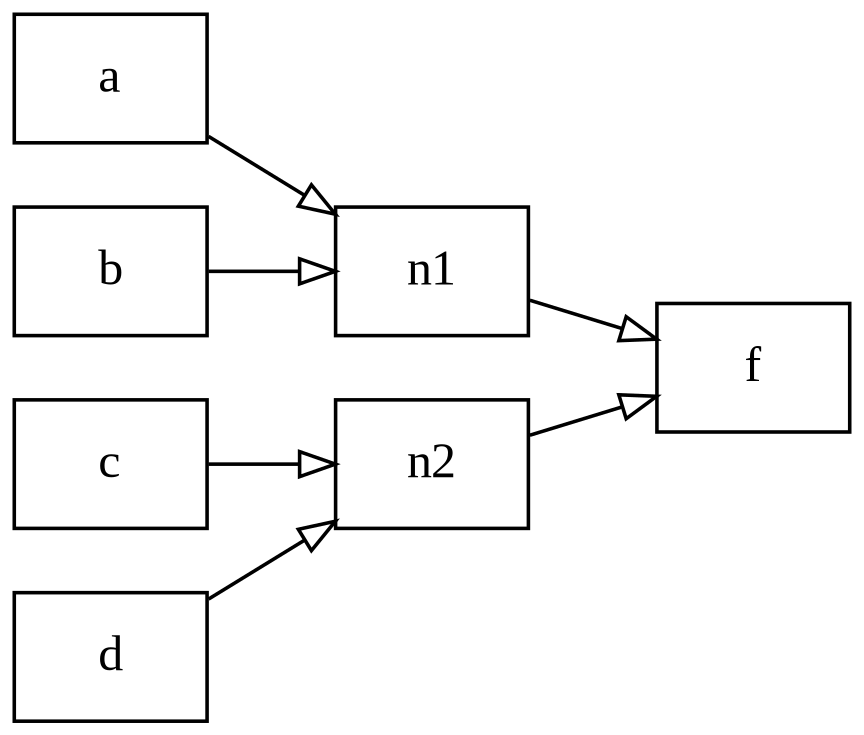
\includegraphics[width=.55\textwidth]{single-elim.png}
  \caption{A single elimination tournament with 4 teams.}
  \label{fig:single-elim}
\end{figure}

\begin{figure}[ht]
  \centering
  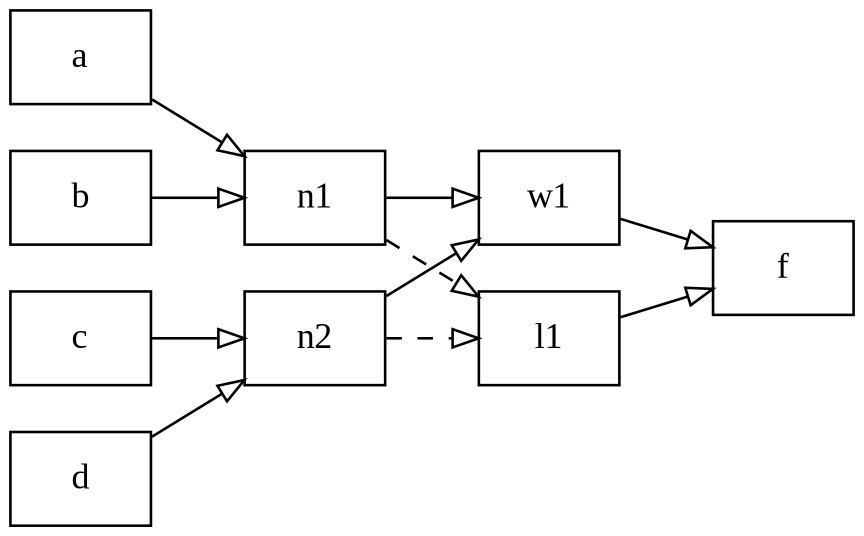
\includegraphics[width=.75\textwidth]{double-elim.png}
  \caption{A simple tournament with a losers bracket. The dashed line represents the loser of that match. So, in this
  case, the losers of \texttt{n1} and \texttt{n2} will play each other in the match \texttt{l1}.}
  \label{fig:double-elim}
\end{figure}

A graph is a collection of nodes, and the relationships between those nodes, called edges. A directed graph is a graph
where the edges, here called arcs, have a direction. For example, in Figure~1 there is an arc from \texttt{a} to
\texttt{n1}, but not vice versa. A directed acyclic graph (DAG) is a special kind of directed graph which has no cycles. A
graph has a cycle if starting from some node, there is a set of edges which will lead to the same node. Alternatively,
a directed graph is acyclic if some node $a$ can be reached from $b$ implies that $b$ can't be reached from $a$.

The number of edges (or arcs) connected to a node is known as the degree of the node. The number of arcs pointing to a
node is known as the in-degree, and the number of arcs pointing away from a node is known as the out-degree.

A phylogenetic tree is a DAG with 2 kinds of nodes: tips, which have in-degree 0; and inner nodes which have in-degree
2. Furthermore, all nodes in a phylogenetic tree have out-degree 1, with one node having out-degree 0. This particular
node is known as the root.

A set of events which time based dependencies, (I.E. one event must be finished before another event) is naturally
acyclic. For example, in a tournament the winner of the two semi-finals must be determined before the winner of the
finals can be determined. Since a tournament is also directed, it is a DAG, as can be seen in
Figures~\ref{fig:single-elim} and \ref{fig:double-elim}.

Similar to a phylogenetic tree, tournaments have 2 types of nodes: competitors which have in-degree 0; and matches,
which have in-degree 2. In contrast with a phylogenetic tree, however, nodes are allowed to have an out-degree of either
1 or 2. This extra out-degree is to account for the loser of a match moving down to a lower bracket. A tournament
retains the special node, or match, with out-degree 0. This is the final match, the one that will decide the winner
of the tournament.

The difference in phylogenetic trees and tournaments does add a complication. When computing the probability of a
particular winner of a particular match we must account for all the possible paths that could have been taken by that
particular team to the particular match. For example, in Figure~\ref{fig:double-elim}, competitor \texttt{a} can arrive
at match \texttt{f} via match \texttt{w1} or via \texttt{l1}. So, in order to accurately compute the probability of
competitor \texttt{a} winning match \texttt{f}, we need to add probability of arriving via \texttt{w1} and \texttt{l1}.

Fortunately, If we account for all possible paths at every node, we only need to worry about the two matches immediately
preceding any given match. We can do this if we make the assumption that the probability of winning a match is ``path
independent''. Such an assumption allows us to ``forget'' about the previous matches that a competitor might have played
in, and restricts the calculation to the match at hand. Please see Section~\ref{sec:theory} for the full details.

\section{Method}

First, we will discuss the theory behind the computation of the single match's distribution of winners in the theory
section. Then, we will discuss how we use this theory to efficiently compute the distribution of winners for a general
tournament, and the software tool that implements this method. Finally, we discuss how we performed our predictions for
the UEFA European Football Championship.

\subsection{Theory}\label{sec:theory}

Some preliminary definitions. The win probability vector (WPV) for a given node is a vector containing the probabilities
of observing a given competitor at that node. We denote the probability of team $a$ winning over team $b$ in a single
match as 

\begin{equation*}
\beats{a}{b}
\end{equation*}

which should be read as ``the probability that team $a$ beats team $b$''. As such, a general WPV has $n$ entries, where
$n$ is the number of teams in the competition.

Suppose that we have a simple tournament, which is just two teams, $a$ and $b$. Then, the WPV which summarizes this
tournament is described by 

\begin{equation}
R_a = \beats{a}{b}, R_b = \beats{b}{a}
\label{eq:base}
\end{equation}

Because this is a trivial case, it is clear that the calculation is easy. For the interest of future examples though,
let us embellish this expression a little bit. First, lets introduce the WPVs for $a$ and $b$ as $w$ and $y$. Since $a$
and $b$ are ``tips'', we just set the probability of observing the team at that node to 1 for the team, and 0 everywhere
else. Then, we get the expression

\begin{equation}
R_a = (\beats{a}{b} \times y_a + \beats{a}{b} \times y_b) \times w_a.
\label{eq:embelished}
\end{equation}

We define $\beats{t}{t} = 0$ for any team $t$. So, because $\beats{a}{a} = 0$ and $y_b = 1$, we can reduce
Equation~\ref{eq:embelished} to Equation~\ref{eq:base}. Using this insight, we can build a general expression for the
WPV on a single elimination tournament as

\begin{equation}
  R_i = w_i \times \sum_{c\in C} \beats{i}{c} \times y_c.
\end{equation}

For multi-elimination tournaments, we need to account the fact that a competitor can come from both sides of the
tournament. Therefore, we need to add a second term to the expression for the other side:

\begin{equation}
  R_i = \left(w_i \times \sum_{c\in C} \beats{i}{c} \times y_{c|i} \right) +
        \left(y_i \times \sum_{c\in C} \beats{i}{c} \times w_{c|i} \right).
        \label{eq:final}
\end{equation}

We calculate $w_{c|i} = w_{c}/(1 - w_i)$, and it should be thought of as the probability of observing competitor $c$ at
$w$ given that competitor $i$ is the other member of the match. So, Equation~\ref{eq:final} is the full general
expression for the WPV of a multi-elimination tournament. The final complication is that $\beats{a}{b}$ might be a
``best of $n$'' series of matches, which will vary over the tournament (early matches are often only a "best of one",
whereas later matches might be a "best of 5"). This can be dealt with by computing a new $P'$ which is the pairwise
probability of winning the ``best of $n$''.

\subsection{Implementation}

In order to compute the most likely winner of the entire tournament, we need to compute the WPV for the final match. For
example, in Figure~\ref{fig:single-elim}, the match \texttt{f} must be evaluated. However, in order to do that, the WPV
for matches \texttt{n1} and \texttt{n2} must be computed, as these are the intermediate results used in
Equation~\ref{eq:final}. Similarly, for the tournament in Figure~\ref{fig:double-elim}, the WPV for matches \texttt{n1}
and \texttt{n2} must be evaluated before the WPV for either match \texttt{w1} or \texttt{l1} can be computed.

Therefore, the tournament matches must be evaluated in the correct order to ensure the correct result. This is analogous
to how a likelihood is computed with a phylogenetic tree, but the key difference here is that there are multiple paths
that a competitor might take to reach the final match. Instead, we need to find a topological sorting of the tournament
DAG. A topological sorting is list of the nodes of a DAG such that, if the list is read left to right, all the
dependencies are satisfied. 

An important detail is how to obtain the win probabilities $P$. In the previous section, this was, intentionally, left
as a black box. This is for two reasons: first, there are many possible ways to compute $P$, and all have their
advantages; and second, it is outside of the scope of this work. Here, we want to focus on two points, the similarity
of phylogenetics to tournaments, and the computation saved from this method.

The complexity of a naive evaluation is $\mathcal{O}(n2^{n}))$ floating point operations. In contrast, the
complexity of a Phylourny like method is $\mathcal{O}(n^2)$. The full proof is quite involved, so it has been relegated
to the supplemental materiel, but we can provide a quick sketch here. Consider the probability that competitor 1 wins in
a 8 competitor single elimination tournament. A \textit{single} term for \textit{just one team} is

\begin{align*}
  &\beats{1}{2} \times \beats{3}{4} \times \beats{5}{6} \times \beats{7}{8} \times \\
  &\beats{1}{3} \times \beats{5}{7} \times \\
  &\beats{1}{5}.
\end{align*}

We have organized the term into layers, one for each ``tier'' of the tournament. Since we start with $n/2$ matches, and
halve every time, we have a known series which sums to $n$. Now, to count the number of terms, we note that we have a
``choice'' for every factor that does not involve competitor 1. For example, we also need to compute the term where
competitor 4 beats competitor 3. This means that there are $2^n - \log(n)$ terms. If we combine these we get the total
expression $n \times (2^n - \log(n) = \mathcal{O} (n2^n)$.

The complexity of a Phylourny like method is much easier to compute. Just note that since we reuse intermediate results
from each match, we just need to evaluate the WPV for each match once. Additionally, there are $n$ elements to the WPV.
So, we need to compute $n$ values per $\mathcal{O}(n)$ matches. This leaves us with the complexity of
$\mathcal{O}(n^2)$.

\subsection{Software}

A reference implementation of the algorithm written in C++ can be found on
GitHub\footnote{\url{https://github.com/computations/phylourny}}. This is also the tool that was used to compute the
predictions in Section~\ref{sec:prediction}. The software only requires CMake to build, and is released under the GPL
version 3.0 license.

\subsection{Prediction of the UEFA Euro 2020}\label{sec:prediction}

In order to predict the winner of the 2020 UEFA European Football Championship, we need to estimate the pairwise win
probabilities of the competing teams. This is challenging, as these teams are assembled for this competition, and have
not played together before this championship. This makes finding data difficult. However, as we are only interested in
verifying our method for \textit{tournaments} we can use the match history from the group stages. Therefore, the
prediction for the winner of the championship was made after the group stage, but before the knockout stage.

Nonetheless, even with match history from the group stage, the data are sparse. Many teams will not play each other
before the group stage, so estimation of pairwise win probabilities is still difficult. To overcome this challenge, we
use two methods. First, we perform a Bayesian sampling of plausible pairwise win probabilities, given the data from the
group stage. The second is to utilize the power of betting markets to estimate the win pairwise probabilities.

The Bayesian sampling is performed via an Markov Chain Monte Carlo (MCMC) search. A pairwise win probability matrix is
proposed, and the associated WPV is computed for the tournament. Additionally, the likelihood of the win probability
matrix is computed using the match data from the group stage. Normally, this process is continued until an event called
``convergence'' occurs.  However, determining when convergence has happened is difficult, so we opt instead to preform a
fixed number of samples.  We feel this is justified, as the state space for \texttt{this} tournament is not excessively
large.

Once we have the samples from the MCMC search, we can compute two predictions: the maximum posterior prediction (MPP),
or the maximum marginal posterior prediction (MMPP). The MPP is simply the prediction from the pairwise win probability
matrix with the highest likelihood, whereas the MMPP is the average prediction from all the samples, weighted by
likelihood. The difference between these two predictions is more of philosophy than mathematics, as they have differing
claims about what ``really'' matters. The school behind the MPP claims that the only thing that matters is the
\textit{most likely} outcome, regardless of distribution, whereas the school behind the MMPP claims that the
\textit{totality of evidence} is what matters. Discussion about the merits of these two schools of thought is beyond the
scope of this paper, however. We instead encourage interested readers to read \textbf{FIND SOME PAPERS FOR THIS}.

Nonetheless, there are 3 predictions: Betting Markets, Maximum Posterior Prediction, and Maximum Marginal Posterior
Prediction. The prediction for each of these methods is summarized in Table~\ref{table:predictions}.

\section{Results}

\begin{table}[ht]
  \centering
  \begin{tabular}{l || r}
    Prediction Method & Winning Team\\
    \hline
    Betting Markets & \\
    Maximum Posterior Prediction & \\
    Maximum Marginal Posterior Prediction & \\
    Actual Result & \\
  \end{tabular}
  \caption{Table of prediction methods, the prediction induced by that method, and the actual result.}
  \label{table:predictions}
\end{table}


\textbf{Ben: I feel that there should be more here than the tournament predictions, but I can't think of what would be
convincing to readers. Any ideas? I suppose we can add these in after the tournament, so we shouldn't feel the need to
have insane time pressure. Also, it might be interesting to try to characterize how ``unstable'' a tournament is if the
win-rates are really equivalent.}

\section{Conclusion}

We have shown that the problem of computing tournament winners is sufficiently close to phylogenetic model likelihood
calculation that many of the same techniques can be applied. We have demonstrated this by developing methods inspired by
phylogenetics which can be applied to tournaments, and that applying these methods corresponds to a large theoretical
speedup. Furthermore, we demonstrate the correctness of these new methods by implementing them into a new software tool
called Phylourny.

As we are writing this \textit{before} the tournament has finished, we don't know how successful our method is at
predicting the true outcome of the result. However, we can still talk about theoretical shortcomings which are true,
even in the case that we predict correctly. There are 2 major shortcomings to this method. First, nearly all the
prediction ``difficulty'' is distilled into estimating the pairwise win probability matrix. However, this is truly the
central problem of tournament prediction, which we don't claim to directly tackle. Instead, we present a
\textit{computational} method, which will accelerate the computation of win probabilities, given some estimation of win
probabilities.

Second, the assumption of path independence might not be true, as competitors might suffer from fatigue from competing
in more matches, if a team must proceed through the lower bracket in order to reach the finals. Furthermore, other
``intangibles'', such as moral or confidence, are hard to quantify in terms of effect, also questioning the path
independence assumption. Nonetheless, these path dependence ostensibly can be solved via a more clever method of
calculating the pairwise win rate matrix, as we can have match dependant $P$. 

While we consider this work more or less complete, there are still further areas of investigation that can be explored.
An example is exploring the ``stability'' of tournaments by slightly varying $P$ and examining the resulting
probabilistic outcome. Another area of interest would be to develop further the MCMC sampling. We currently have an
extremely naive implementation of an MCMC search, but this can be made much more efficient by specifying an appropriate
method of proposing parameters.

\bibliography{references}
\bibliographystyle{acm}

\end{document}
